\section{Thrust 4. AI-Powered Learning Environment in Programming for VIPLs}
\label{sec:thrust4}

\begin{wrapfigure}{r}{3.5in}
\centering
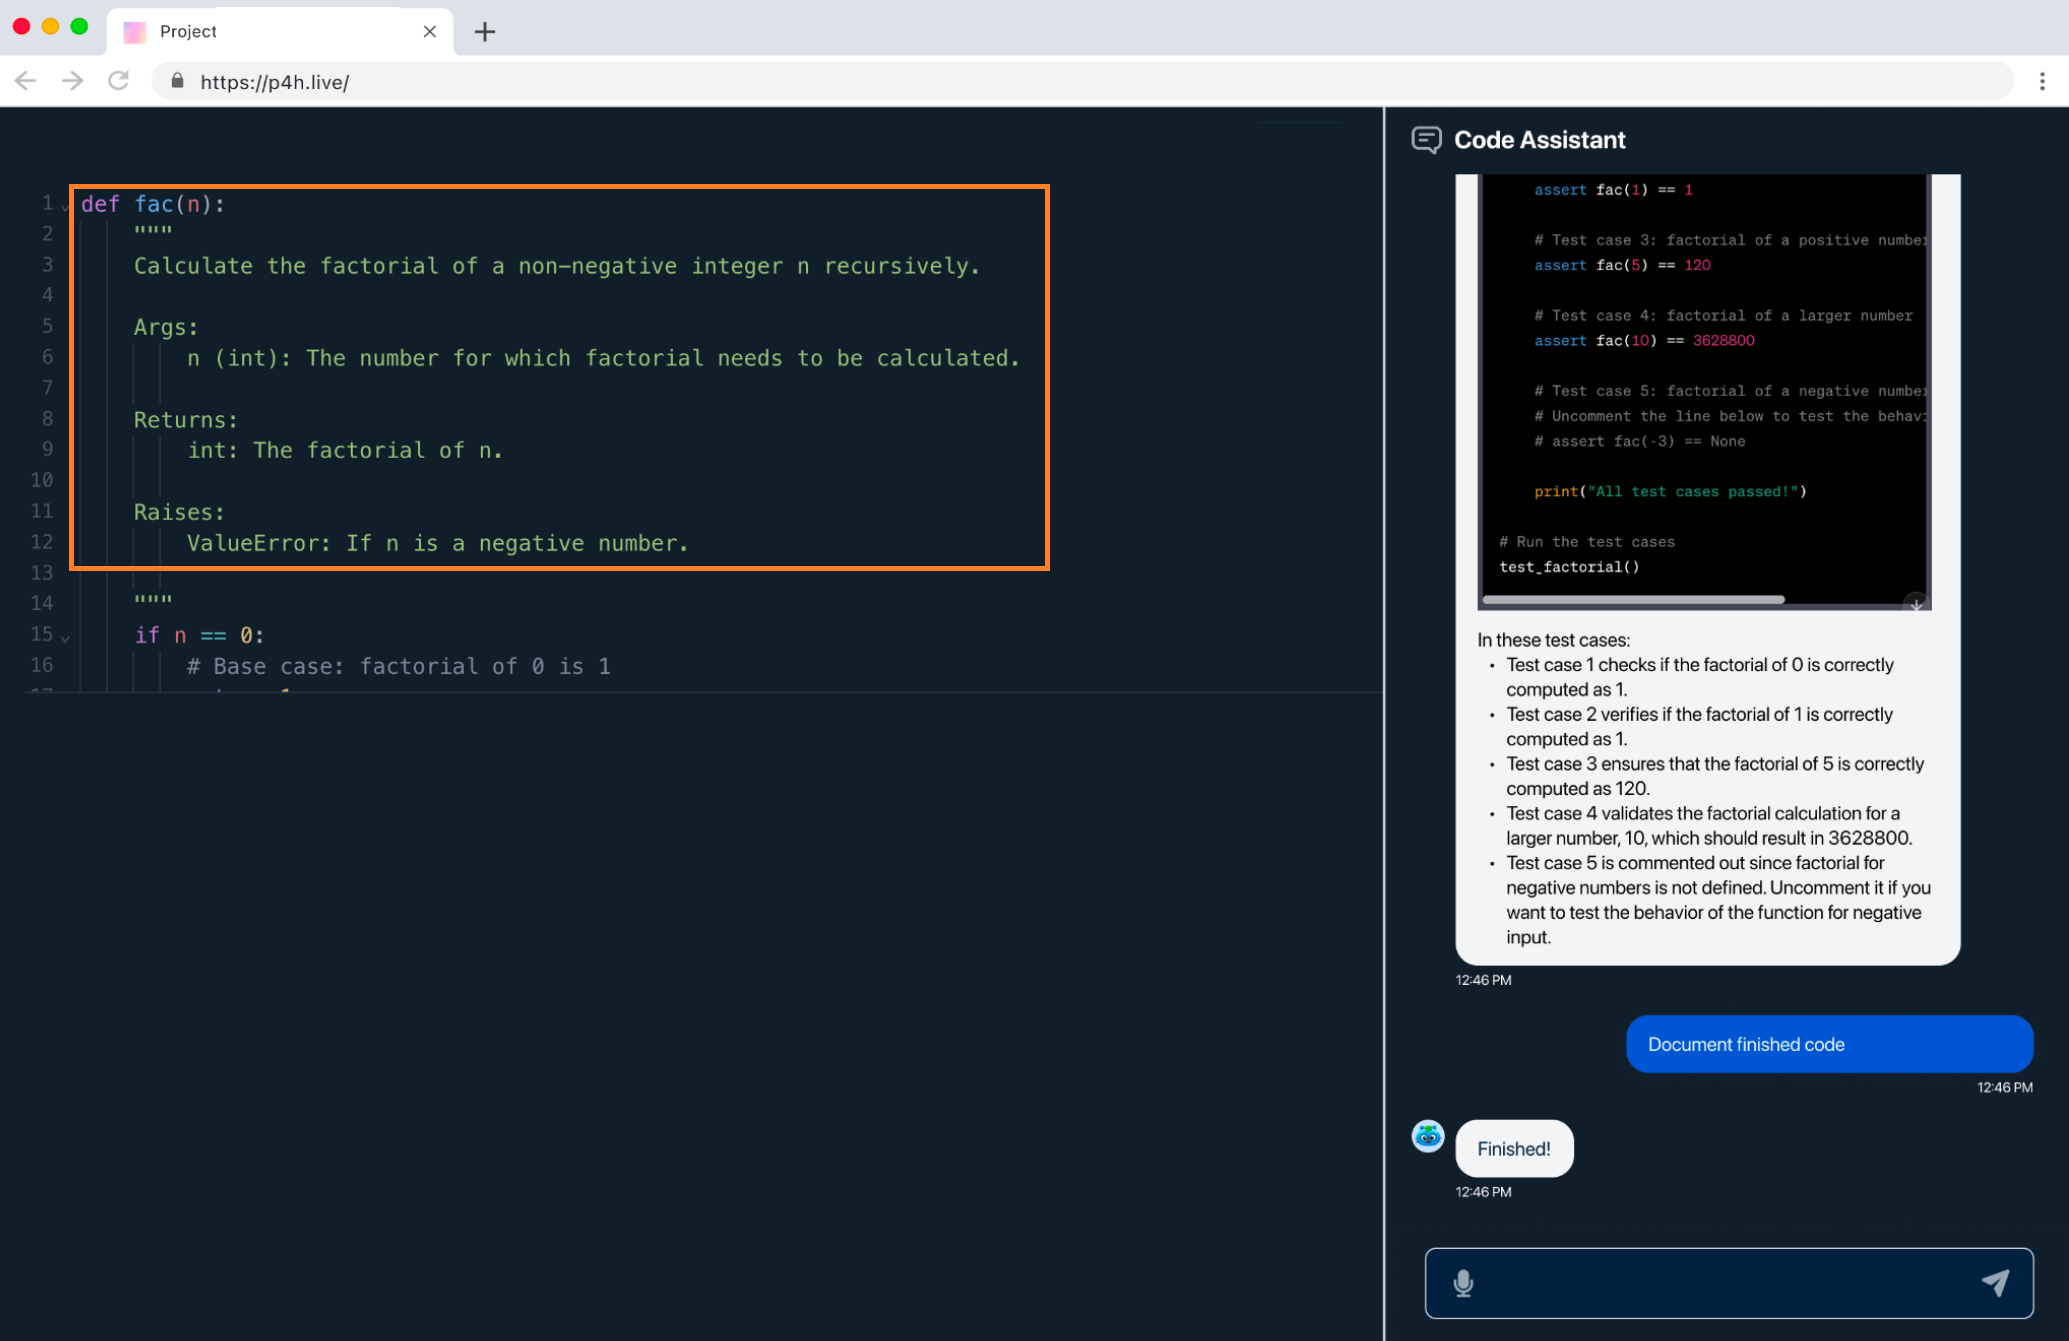
\includegraphics[width=3.4in]{p4h-7}
\vspace{-6pt}
\caption{Tutorial and Learning Environment for VIPLs}
\label{auto-doc}
\end{wrapfigure}

Introducing a tutorial learning environment that revolutionizes the way visually-impaired learners engage with programming. Tailored to meet the unique needs of this community, this platform employs state-of-the-art Voice to Text and Text to Code technologies, ensuring an accessible and immersive learning experience. Through Voice to Text, students can articulate their ideas and queries naturally, with the platform converting spoken language into precise, contextually-rich text. This feature's adaptability accommodates various accents and speech patterns, making it inclusive for a diverse global audience. Complementing this, the Text to Code functionality takes learning to the next level. Driven by advanced natural language processing, it interprets human-readable instructions and descriptive language, seamlessly generating accurate and syntactically correct code snippets.

%This powerful capability empowers visually-impaired learners to code fluently, breaking down barriers and unleashing their full potential in the world of programming.

Within this tutorial environment, every step is meticulously designed to ensure maximum comprehension and engagement. Rich audio cues provide real-time feedback, reinforcing learning and enhancing understanding. Text descriptions are supplemented with auditory explanations, creating a multi-modal learning experience that caters specifically to the needs of visually-impaired students. Furthermore, tactile interfaces are integrated, offering haptic feedback to reinforce key programming concepts. The environment's intuitive navigation and user-friendly interface make it easy for learners to progress through tutorials at their own pace, building a solid foundation in programming. With a focus on accessibility and innovation, this tutorial learning environment empowers visually-impaired learners to excel in the world of coding, opening up new possibilities and opportunities for a more inclusive tech community.
